\documentclass{article}[]

\usepackage[utf8]{inputenc}
\usepackage{graphicx}
\usepackage[catalan]{babel}
\usepackage{dirtytalk}
\usepackage{titlesec}
\usepackage[hidelinks]{hyperref}
\usepackage[T1]{fontenc}

\setlength{\parindent}{0pt}

%----------------------------------------------------------------------------------------
%	TITLE PAGE
%----------------------------------------------------------------------------------------

\newcommand*{\titleGM}{\begingroup % Create the command for including the title page in the document
\hbox{ % Horizontal box
\hspace*{0.2\textwidth} % Whitespace to the left of the title page
\rule{1pt}{\textheight} % Vertical line
\hspace*{0.05\textwidth} % Whitespace between the vertical line and title page text
\parbox[b]{0.75\textwidth}{ % Paragraph box which restricts text to less than the width of the page

{\noindent\Huge\bfseries AndroShopping \\}\\[2\baselineskip] % Title
{\large \textit{Llenguatges de Programació \\\\ 2014 - 2015}}\\[4\baselineskip] % Tagline or further descriptio


\vspace{0.5\textheight}
\begin{flushright}
Albert Lloveras (ls27332)\\
Manel Roca (ls27599)
\end{flushright}
{\noindent}
\\[\baselineskip] % Publisher and logo
}}
\endgroup}

%----------------------------------------------------------------------------------------
%	BLANK DOCUMENT
%----------------------------------------------------------------------------------------

\begin{document}

\pagestyle{empty} % Removes page numbers

\titleGM % This command includes the title page

\tableofcontents

\newpage
\pagestyle{plain}


\section{Introducció}
Aquest any a l'assignatura de llenguatges de programació ens han encarregat el desenvolupament d'una App per a sistemes Android per gestionar les compres d'una botiga.\\

En quant a requeriments, ens han demanat que l'aplicació sigui capaç de sincronitzar les seves dades amb una base de dades a la qual accedirem a través d'un WebService. Per ser més concisos, l'adreça del WebService que se'ns ha proporcionat és:\\

\begin{center}
\url{http://www.v2msoft.com/curso-android/ws/}
\end{center}

De l'anterior WebService se'ns han proporcionat les següents rutes:
\begin{itemize}
	\item  \textbf{http://www.v2msoft.com/curso-android/ws/last\_update.php}:\\
	Aquesta ruta ens permet conèixer la data de la última modificació de la Base de Dades (en format JSON) per tal de determinar si cal o no descarregar-nos de nou les dades al terminal mòbil.
	\item \textbf{http://www.v2msoft.com/curso-android/ws/lista\_productos.php}:\\
	Aquesta ruta ens retorna un array d'objectes JSON que representen els productes disponibles per la venda al nostre establiment.
\end{itemize}

A l'hora de parlar de funcionalitats de la nostre App, hem de definir primerament que l'aplicació tindrà un seguit d'usuaris els quals podran tenir dos rols:
\begin{itemize}
	\item Rol usuari:\\
	Aquest tipus d'usuari serà el bàsic de la aplicació i només podrà realitzar operacions de modificació del seu perfil, realitzar compres dels productes disponibles a l'establiment i consultar el seu històric de compres realitzades.
	\item Rol admin:\\
	Aquest tipus d'usuari estarà reservat només als responsables de l'establiment. D'aquesta manera, les funcionalitats que presenta són lleugerament diferents a les citades anteriorment. Per ser més concrets, aquest rol d'usuari permetrà manegar els usuaris de la aplicació, manegar els productes de l'establiment i tenir un seguiment de totes les ventes realitzades amb la possibilitat de consultar quin client ha fet cada compra.
\end{itemize}

Finalment, cal destacar que els requeriments tècnics a nivell de Android són que la nostre App ha de ser compatible amb la SDK 15 en amunt i una versió de Android 4.4.0 o superior. No obstant, se'ns ha demanat un disseny i programació optimitzats per a la SDK 22 i versió de Android 5 o superior. 


\section{Diagrama de classes}

\begin{center}
	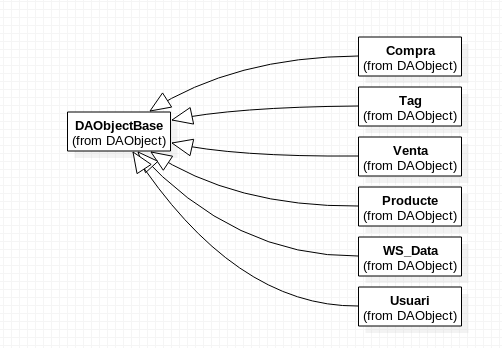
\includegraphics[scale=0.5]{img/1.png}
	 \end{center}
		El conjunt de classes anteriors representen els objectes utilitzats per tal de gestionar les dades de la base de dades.

Aquests objectes contenen els mateixos atributs que la taula corresponent a SQLite.

La seva utilitat és persistir en memòria principal la informació recuperada de la base de dades i poder operar amb aquesta.

Tots els objectes utilitzats en aquest paquet hereten de DAObjectBase, que bàsicament conté l'atribut id, comú en tots els objectes de la base de dades.
	\begin{center}
	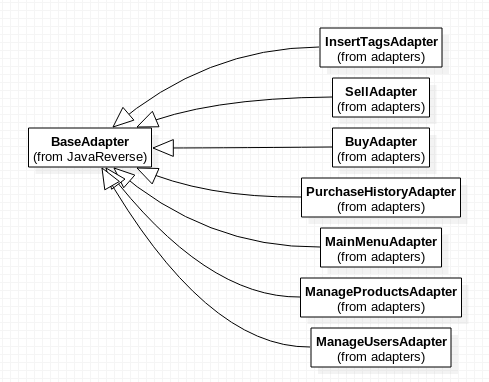
\includegraphics[scale=0.5]{img/2.png}
	 \end{center}
	 
	 \newpage
	 	 Tal i com es pot apreciar a la imatge anterior, per a la realització de la nostre pràctica, ens hem ajudat dels adapters per tal d'inflar de forma dinàmica i eficient diversos Layouts o ListViews.\\
	
	Per fer-ho, hem hagut d'heretar d'una de les classes base d'Adapters que proporciona Android que, en el nostre cas, ha estat la classe BaseAdapter.
	 \begin{center}
	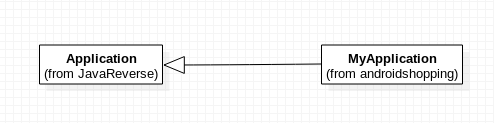
\includegraphics[scale=0.5]{img/3.png}
	\end{center}
	L'objectiu de l'herència anterior i de la classe MyApplication és tenir un \textit{singleton} que permeti la persistència d'informació en memòria al llarg de la vida de la nostre aplicació. Un exemple del contingut desat en aquest \textit{singleton} són els identificadors únics dels \textit{mutex}.
	\begin{center}
	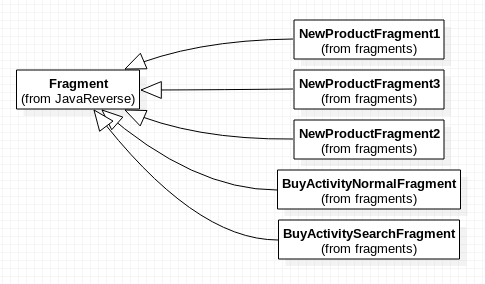
\includegraphics[scale=0.5]{img/4.png}\\
\end{center}
	Per tal d'encarar moltes de les vistes de la nostre aplicació hem decidit fer ús de Fragments.És per això que, en la il·lustració anterior es mostren totes les classes JAVA corresponents a la lògica d'aquests fragments.\\
	
	Com es pot apreciar, totes les classes dels nostres fragments, hereten de la classe Fragment que proporciona Android. D'aquesta manera, podem fer que dins d'una mateixa activitat, se'ns canviï el contingut mostrat a l'usuari, sense necessitat de carregar una altra activitat o quadre de diàleg.\\
\begin{center}
	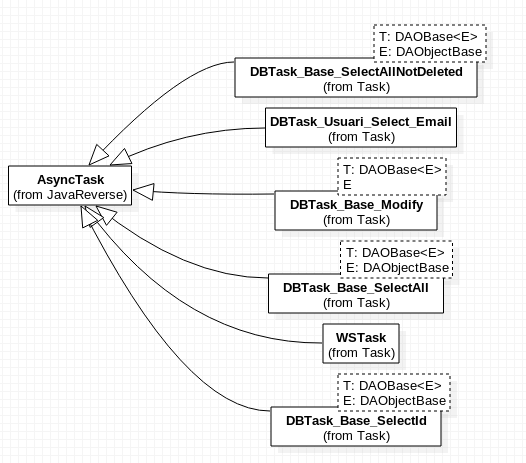
\includegraphics[scale=0.5]{img/5.png}
	\end{center}
	La gestió d'informació amb la base de dades, tant per consultar, com per modificar les dades, havia d'estar en un thread independent del thread que controla les vistes de l'aplicació. Aquest requeriment és degut al fet que mentre s'executen les comandes amb la base de dades, l'aplicació no podria gestionar els elements visuals que es mostren a l'activitat. Per solucionar aquest problema es genera una AsyncTask quan es vol interactuar amb la base de dades.\\

Aquesta interfície de comunicació amb les dades s'ha fet creant classes que heretaven de la classe AsyncTask. Es va intentar crear una AsyncTask personalitzada per cadascuna de les funcionalitats que es podien realitzar.\\

La majoria de classes d'aquest grup són Templates. Això vol dir que creant una sola classe es podia utilitzar per diversos tipus de dades diferents. Per realitzar això el que es va fer és definir un Tipus T que havia d'heretar del DAOBase. La classe DAOBase té els mètodes abstractes que han d'implementar totes les classes DAO que deriven d'aquesta. D'aquesta manera es podia cridar als diferents mètodes dins de l'AsyncTask. També es va definir un tipus E que heretava del DAObjectBase, per tal de passar a l'AsyncTask el tipus de dada on s'ompliria el contingut de la consulta.
	\begin{center}
	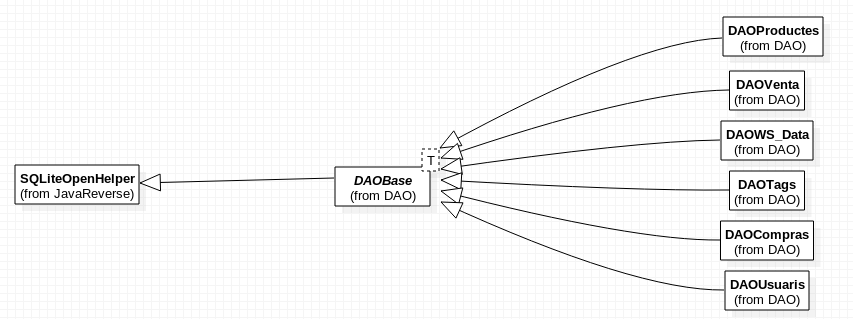
\includegraphics[scale=0.5]{img/6.png}
	\end{center}
Les classes amb el prefix DAO serveixen com ha connexió entre les dades de la base de dades i les dades carregades en memòria.

Aquestes classes fan tenen els mètodes necessaris per moure la informació d'un costat a un altre. Totes hereten de DAOBase que té, com s'ha comentat abans, els tots els mètodes bàsics que han d'implementar les diferents classes. Totes elles acaben hereten de SQLiteOpenHelper, una classe d'Android.

Les operacions més bàsiques són: select by id, select all, insert, update i delete.
	\begin{center}
	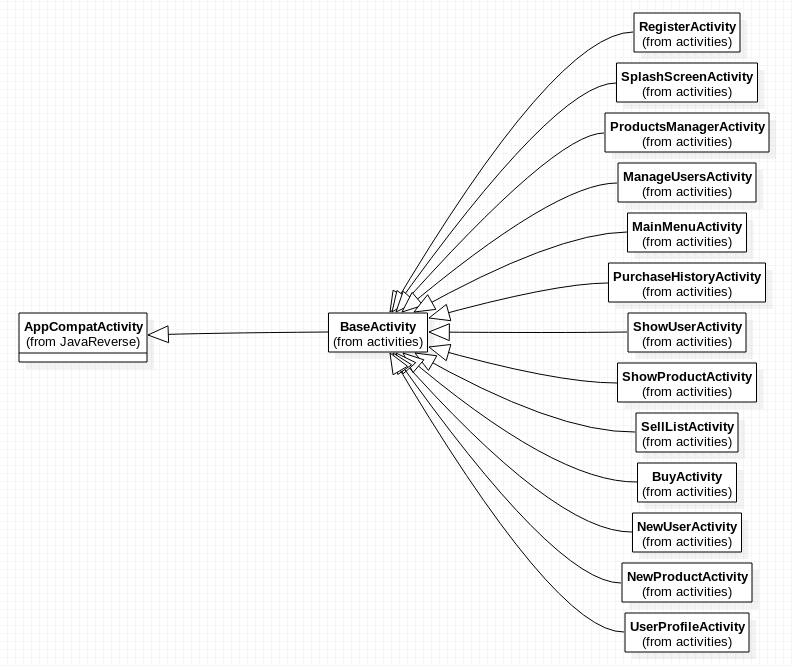
\includegraphics[scale=0.5]{img/7.png}
\end{center}
	Finalment, a l'hora d'organitzar les classes que fan referència a les activitats de la nostre aplicació, vàrem creure oportú definir una classe base \textit{BaseActivity} la qual definís les característiques principals i comunes a cada activitat (per poder-les heretar) així com també implementar mètodes per realitzar tasques comunes a les activitats, com per exemple, mètodes que permetessin l'intercanvi de fragments, l'actualització d'informació a la \textit{ActionBar...}
	
\begin{center}
\end{center}
\newpage
\section{Diagrama BBDD}
\begin{center}
	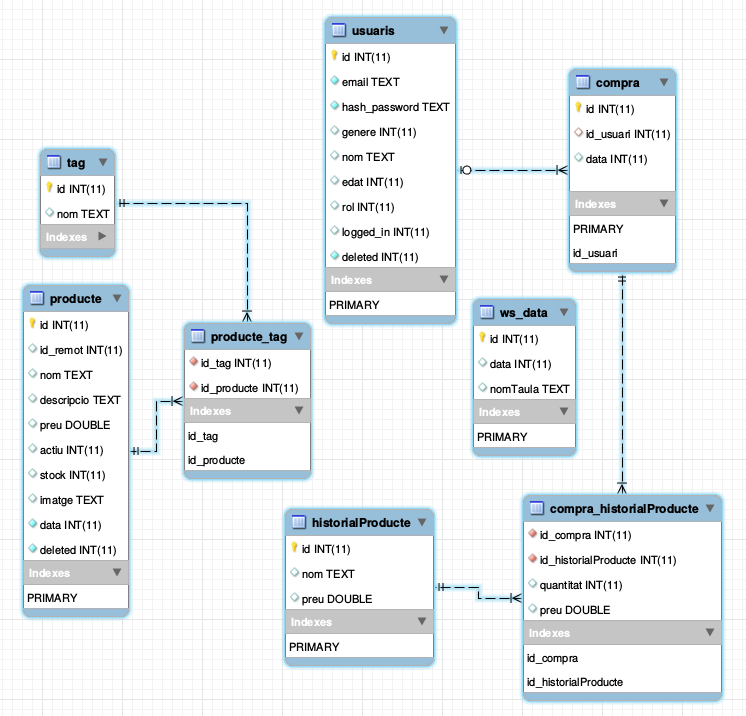
\includegraphics[scale=0.5]{img/Android_DB_Schema.png}
\end{center}
La nostra aplicació necessita persistir les dades en memòria un cop es tanca, així que s'ha utilitzat un sistema de bases de dades natiu d'Android, SQLite.\\

Per resoldre la pràctica s'han utilitzat les taules que es mostren a la figura anterior.\\

En primer lloc tenim la taula usuaris que guarda el correu i la contrasenya dels usuaris. Aquesta informació s'utilitza posteriorment per verificar i controlar l'accés a l'aplicació. El camp contrasenya utilitza la codificació SHA-256 per encriptar les dades.\\

\newpage

La taula usuaris es relaciona amb la taula compra que serveix per emmagatzemar les diferents operacions de compra que realitza l'usuari.\\

La taula producte guarda la informació recuperada del WS i creada per l'usuari. Aquesta taula es relaciona amb la taula tag a través de la taula relacional producte{\_}tag. Dins la mateixa taula producte no es podia guarda la id que es proporcionava com a identificador de la fila, ja que al poder generar informació des de dues opcions diferents, podien col·lidir els identificadors. Es va solucionar el problema creant un identificador únic per la nostra base de dades local i emmagatzemant la id del servidor remot en una columna anomenada id{\_}remot.

\section{Conclusions}
Les conclusions de la realització d'aquesta pràctica de llenguatges de programació són:\\

En primer lloc, posar en pràctica, de forma conjunta, tots els conceptes vistos a classe durant el semestre. Això ha servit per veure la potencia real del contingut explicat així com també detectar possibles problemes a l'hora d'integrar diverses funcionalitats vistes a classe en problemes reals (càrrega d'imatges mitjançant asynctasks -> out of memory error).\\

Per ser més concrets, hem practicat i molt tot el tema de concurrència, threads i bases de dades. Això ens ha ajudat a reflexionar sobre la importància de definir-se una bona estructura de classes (DAOs i altres) per tal de fer que l'accés a la BBDD sigui prou còmode i escalable, ja que no saps mai, en un futur, quins canvis et poden demanar.\\

Per altra banda, hem descobert i aprés a utilitzar Picasso, que ens ha ajudat moltíssim a gestionar l'accés a les imatges que s'havien de mostrar en les pantalles de la nostre aplicació.  A més a més, hem utilitzat la llibreria Jackson per tal de fer-nos més fàcil la interacció amb els valors de retorn del WebService. 

Per si tot això fos poc, a nivell de programació multiprocés i concurrent, hem aprés a sincronitzar diferents threads mitjançant l'ús de listeners i interfícies.

Finalment, destacar que la realització d'aquesta pràctica també ens ha fet acostumar-nos al nou entorn de desenvolupament de Androi (Android Studio), ja que l'any passat vàrem treballar amb Eclipse. A més, dins d'aquests canvis d'IDE ens hem hagut de familiaritzar amb els nous fitxers de configuració de Gradle per tal d'importar les llibreries de manera quasi automàtica.


\end{document}
